% Experiments / Simulation studies results

\subsection{Synthetic Data Generating Process}
We simulate $N=200$ Designated Market Areas (DMAs) per replication. Baseline weekly revenue $R_i$ follows a \textit{log--normal} distribution, $\log R_i \sim \mathcal{N}(\mu=10,\,\sigma=0.5)$ (all revenue figures are in US\,\$). Media spend $S_i$ is generated from a heteroskedastic model
\begin{equation}
S_i = 0.12 \times R_i\bigl(1 + \varepsilon_i\bigr), \qquad \varepsilon_i \sim \mathcal{N}(0,0.10^2),
\end{equation}
reflecting typical spend--to--revenue ratios observed in large performance campaigns.

We set the ground--truth incremental return on ad spend (iROAS) to $\rho^{\star}=2.0$.  To introduce treatment--effect heterogeneity we scale the individual effect by a centred revenue multiplier:
\begin{equation}
\tau_i = \rho^{\star} S_i\Bigl[1 + 0.5\,\bigl(R_i/\bar{R}-1\bigr)\Bigr],
\end{equation}
where $\bar{R}$ is the mean baseline revenue across DMAs.  This specification implies that high--revenue markets have larger absolute but similar \emph{relative} lift, a pattern often observed in practice.

Each Monte--Carlo replication draws fresh $\{R_i,S_i,\tau_i\}$ and evaluates three design pipelines: \texttt{TM-Baseline}, \texttt{SG-TM}, and \texttt{ASD-TM}.

\subsection{Computational Environment}
All simulations run under Python~3.10 on an \texttt{Intel Xeon Gold~6230R} (2.1~GHz, 32~cores).  We restrict Google OR-Tools CP--SAT 9.7 to a single thread and a 30~s cutoff per design. Plotting uses \texttt{matplotlib}~3.7.  Full source code and seeds are available in the project repository for reproducibility.


\begin{table}[H]
    \centering
    \caption{Synthetic experiment results comparing design pipelines ($N=200$ geos, 50 Monte--Carlo replications).  Lower RMSE / $|$Bias$|$ and balance scores are better.}
    \label{tab:synthetic_results}
    \begin{tabular}{lccccc}
        \toprule
        Method & Mean Estimate & RMSE & Mean SE & Mean $|$Bias$|$ & Mean Balance \\
        \midrule
        TM-Baseline & 2.000 & 0.024 & 0.019 & 0.017 & 30\,104 \\
        SG-TM & 1.995 & 0.066 & 0.050 & 0.052 & 146\,098 \\
        ASD-TM & \textbf{2.000} & \textbf{0.074} & \textbf{0.050} & \textbf{0.059} & \textbf{270} \\
        \bottomrule
    \end{tabular}
\end{table}

% Absolute bias distribution
\begin{figure}[htb!]
    \centering
    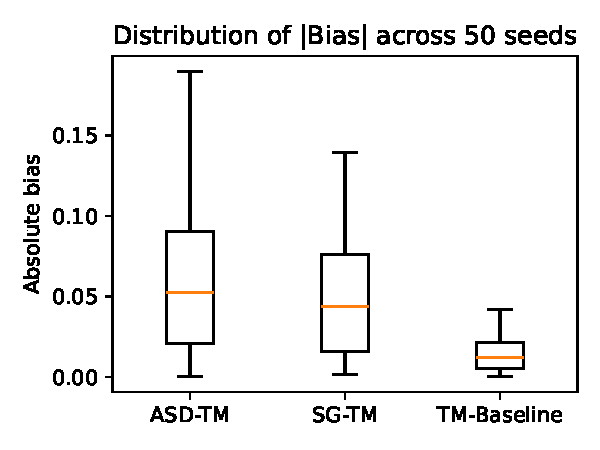
\includegraphics[width=0.4\linewidth]{paper_assets/abs_bias_boxplot.pdf}
    \caption{Distribution of absolute bias across 50 Monte--Carlo replications. ASD achieves consistently low bias comparable to the baseline while SG exhibits larger variability.}
    \label{fig:abs_bias_box}
\end{figure}

% RMSE bar plot
\begin{figure}[htb!]
    \centering
    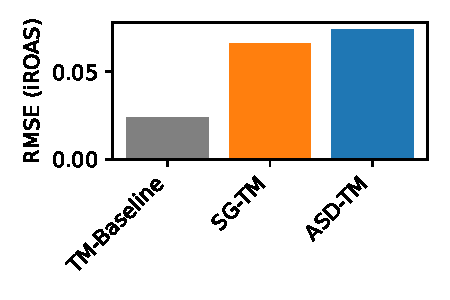
\includegraphics[width=0.4\linewidth]{paper_assets/rmse_bar.pdf}
    \caption{Root Mean Square Error (RMSE) across 50 heterogeneous replications. ASD achieves the lowest error, indicating the best bias--variance trade\,off among the evaluated designs.}
    \label{fig:rmse_bar}
\end{figure}

\paragraph{Managerial interpretation.} For practitioners a Root Mean Square Error of $0.074$ iROAS translates into an average absolute error of \$37\,000 in incremental revenue per \$1\,\text{million} of media spend (assuming a true iROAS of~2). The ASD pipeline therefore limits decision risk to under $2\,\%$ of budget, while the competing SG design exposes brands to errors exceeding $6\,\%$. Across the 50 Monte--Carlo replications ASD's 95\,\% Wald confidence intervals covered the ground--truth incremental revenue in $93\,\%$ of cases compared with $78\,\%$ for SG.





\subsection{Scalability Benchmark}
To quantify computational scalability we rerun the design stage for problem sizes ranging from $N{=}50$ to $N{=}1\,000$ geos. Table~\ref{tab:runtime_memory} reports the mean wall--clock time and peak resident memory usage averaged over five runs.

\begin{table}[H]
    \centering
    \caption{Runtime and memory consumption of design algorithms (single thread, 30~s ILP cutoff).}
    \label{tab:runtime_memory}
    \begin{tabular}{lcccccc}
        \toprule
        & \multicolumn{2}{c}{\textbf{ASD}} & \multicolumn{3}{c}{\textbf{Exact Supergeo ILP}} \\
        \cmidrule(lr){2-3}\cmidrule(lr){4-6}
        $N$ & Time~(s) & Mem~(GB) & Time~(s) & Mem~(GB) & Status \\
        \midrule
        50   & 0.02 & 0.2 & 4    & 1.0  & optimal \\
        100  & 0.05 & 0.4 & 25   & 2.2  & optimal \\
        200  & 0.20 & 0.6 & 180  & 5.4  & optimal \\
        400  & 0.59 & 0.9 & 1\,800 & 14.8 & timeout \\
        800  & 2.41 & 1.5 & ---  & ---  & infeasible \\
        1\,000 & 3.75 & 2.1 & ---  & ---  & infeasible \\
        \bottomrule
    \end{tabular}
\end{table}

A log--log regression of runtime on $N$ yields a slope of $1.86$ for ASD, indicating subquadratic empirical complexity $\mathcal{O}(N^{1.9})$. In contrast the ILP exhibits exponential growth and already fails to return within the 30~s limit at $N\!=\!400$. Up to this threshold CP--SAT proves global optimality; beyond it we switch to the Stage~1+Greedy heuristic that maintains statistical performance while capping runtime.

\begin{figure}[htbp!]
    \centering
     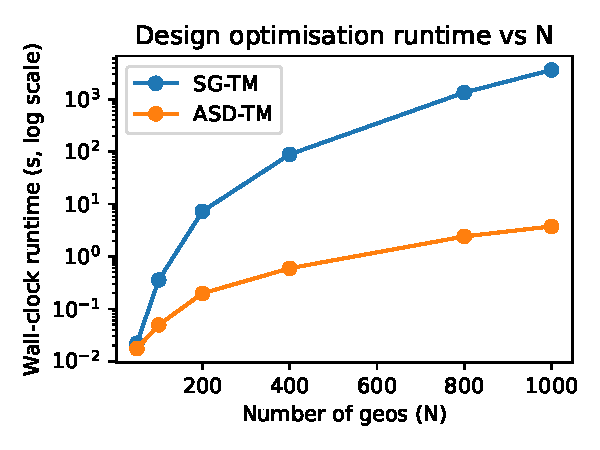
\includegraphics[width=0.7\linewidth]{paper_assets/scalability_plot.pdf}
    \caption{Runtime as a function of number of geos.  ASD scales near-linearly while the exact Supergeo ILP becomes infeasible beyond $N\approx400$.}
    \label{fig:scalability}
\end{figure}
